%!TEX root = DisenoProyecto_LuisGomez.tex

%%!TEX root = DisenoProyecto_LuisGomez.tex

%%!TEX root = DisenoProyecto_LuisGomez.tex

%%!TEX root = DisenoProyecto_LuisGomez.tex

%\input{11_Diagrama_Gantt.tex}

%\begin{consigna}{red}
%
%Existen muchos programas y recursos \textit{online} para hacer diagramas de Gantt, entre los cuales destacamos:
%
%\begin{itemize}
%\item Planner
%\item GanttProject
%\item Trello + \textit{plugins}. En el siguiente link hay un tutorial oficial: \\ \url{https://blog.trello.com/es/diagrama-de-gantt-de-un-proyecto}
%\item Creately, herramienta online colaborativa. \\\url{https://creately.com/diagram/example/ieb3p3ml/LaTeX}
%\item Se puede hacer en latex con el paquete \textit{pgfgantt}\\ \url{http://ctan.dcc.uchile.cl/graphics/pgf/contrib/pgfgantt/pgfgantt.pdf}
%\end{itemize}
%
%Pegar acá una captura de pantalla del diagrama de Gantt, cuidando que la letra sea suficientemente grande como para ser legible. 
%Si el diagrama queda demasiado ancho, se puede pegar primero la ``tabla'' del Gantt y luego pegar la parte del diagrama de barras del diagrama de Gantt.
%
%Configurar el software para que en la parte de la tabla muestre los códigos del EDT (WBS).\\
%Configurar el software para que al lado de cada barra muestre el nombre de cada tarea.\\
%Revisar que la fecha de finalización coincida con lo indicado en el Acta Constitutiva.
%
%En la figura \ref{fig:gantt}, se muestra un ejemplo de diagrama de Gantt realizado con el paquete de \textit{pgfgantt}. En la plantilla pueden ver el código que lo genera y usarlo de base para construir el propio.
%
%\begin{figure}[htbp]
%\begin{center}
%\begin{ganttchart}{1}{12}
%  \gantttitle{2020}{12} \\
%  \gantttitlelist{1,...,12}{1} \\
%  \ganttgroup{Group 1}{1}{7} \\
%  \ganttbar{Task 1}{1}{2} \\
%  \ganttlinkedbar{Task 2}{3}{7} \ganttnewline
%  \ganttmilestone{Milestone o hito}{7} \ganttnewline
%  \ganttbar{Final Task}{8}{12}
%  \ganttlink{elem2}{elem3}
%  \ganttlink{elem3}{elem4}
%\end{ganttchart}
%\end{center}
%\caption{Diagrama de Gantt de ejemplo}
%\label{fig:gantt}
%\end{figure}
%
%
%\begin{landscape}
%\begin{figure}[htpb]
%\centering 
%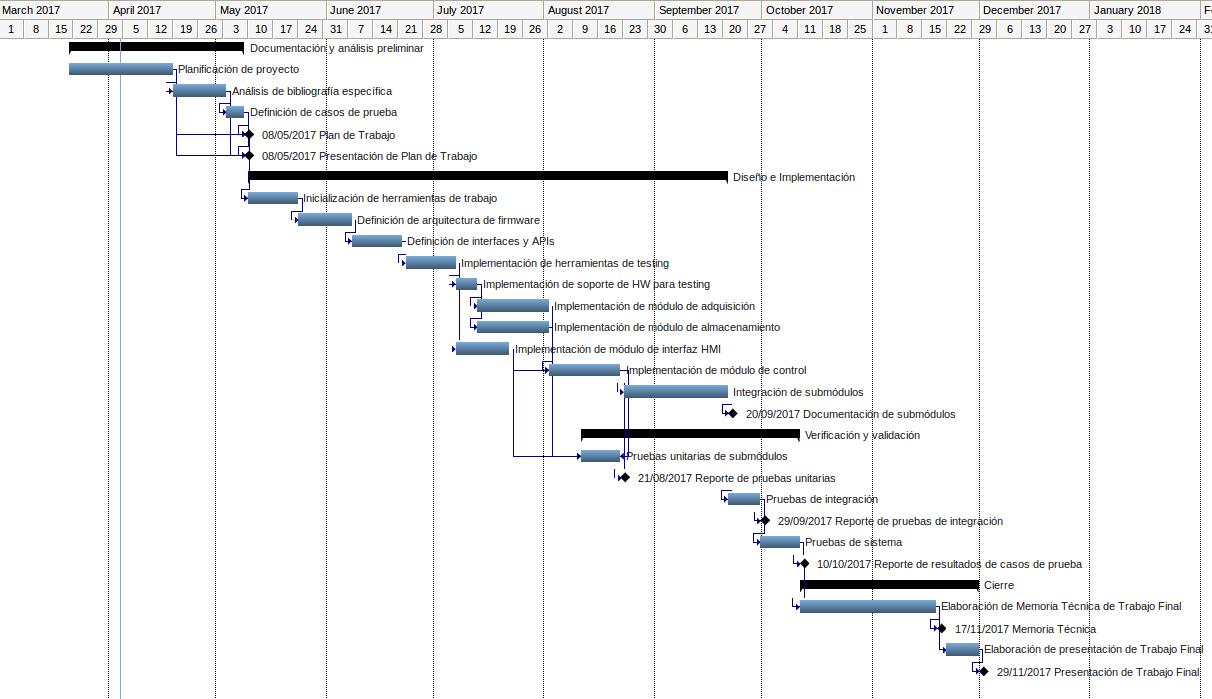
\includegraphics[height=.85\textheight]{./Figuras/Gantt-2.png}
%\caption{Ejemplo de diagrama de Gantt rotado}
%\label{fig:diagGantt}
%\end{figure}
%
%\end{landscape}
%
%\end{consigna}

%\begin{landscape}
\rotatebox{90}{%
\begin{ganttchart}[
	hgrid,
    vgrid={*4{dotted}, *3{red!50}}, %	vgrid,
	x unit=0.12cm,
	y unit chart=0.7cm,
	time slot format=isodate,
	time slot unit=day,
	bar/.append style={fill=blue!30},
	group/.append style={fill=blue!50},
	%link/.style={->, thick}
	]{2023-09-11}{2024-01-24}
	
	\gantttitlecalendar{year, month} \\
			\ganttmilestone{0. Acta de Constitución}{2023-09-11}\\
		\ganttgroup{1 Gestión del Proyecto}{2023-09-11}{2023-10-13} \\
		\ganttbar[name=11]{1.1 Generación de requerimientos}{2023-09-11}{2023-09-15} \\
		\ganttbar[name=12]{1.2 Planificación del proyecto}{2023-09-18}{2023-09-29} \\
		\ganttbar{1.3 Planificación de entregables}{2023-10-02}{2023-10-04} \\
		\ganttbar{1.4 Revisión y ajustes}{2023-10-04}{2023-10-13} \\
			\ganttmilestone{1.5 Proyecto de tesis}{2023-10-13} \\
	
	\ganttgroup{2 Diseño General}{2023-10-16}{2023-11-03} \\
		\ganttbar{2.1 Ajuste al diseño conceptual}{2023-10-16}{2023-10-18} \\
		\ganttbar{2.2 Diagramas de flujo}{2023-10-18}{2023-10-25} \\
		\ganttbar{2.3 Revisión y ajustes de diseño}{2023-10-25}{2023-11-03} \\
	
	\ganttgroup{3 Construcción del hardware}{2023-11-06}{2023-12-15} \\
		\ganttbar{3.1 Selección de componentes}{2023-11-06}{2023-11-10} \\
		\ganttbar{3.2 Diseño de circuitos}{2023-11-13}{2023-11-24} \\
		\ganttbar{3.3 Montaje y soldadura}{2023-11-27}{2023-12-06} \\
		\ganttbar{3.4 Pruebas iniciales}{2023-12-06}{2023-12-15} \\
	
	\ganttgroup{4 Diseño del firmware}{2023-12-18}{2024-01-24} \\
		\ganttbar{4.1 Diseño de arquitectura}{2023-12-18}{2023-12-22} \\
		\ganttbar{4.2 Implementación de MP2,5}{2023-12-25}{2024-01-03} \\
		\ganttbar{4.3 Almacenamiento y comunicación}{2024-01-03}{2024-01-12} \\
		\ganttbar{4.4 Funciones auxiliares}{2024-01-15}{2024-01-24} 
	
	\ganttlink[]{11}{12}
	
\end{ganttchart}
}
\newpage
\rotatebox{90}{%
\begin{ganttchart}[
	hgrid,
%vgrid,
 vgrid={*4{dotted}, *3{red!50}}, %	vgrid,
x unit=0.14cm,
y unit chart=0.7cm,
time slot format=isodate,
time slot unit=day,
bar/.append style={fill=blue!30},
group/.append style={fill=blue!50},
bar/.append style={fill=blue!30, bar label node/.append style={above=3pt}},
%include title in canvas=false,
%inline,
milestone inline label node/.append style={left=5mm}
%link/.style={->, thick}
%link label font=\small\bfseries\color{purple}
link/.style={|-to, line width=0.5pt, blue},
    bar inline label node/.style={
	anchor=east,
	xshift=+4.5cm,
	yshift=0.4cm,
}
]{2024-01-22}{2024-05-28}
	
	\gantttitlecalendar{year, month} \\
	
	\ganttgroup{5 Realización de pruebas}{2024-01-24}{2024-02-21} \\
		\ganttbar[name=51]{5.1 Diseño de casos de prueba}{2024-01-24}{2024-01-31} \\
		\ganttbar[name=52]{5.2 Ejecución de pruebas}{2024-01-31}{2024-02-14} \\
		\ganttbar[name=53]{5.3 Análisis de resultados}{2024-02-14}{2024-02-21} \\
		
	\ganttgroup{6 Ajustes finales}{2024-02-21}{2024-03-06} \\
		\ganttbar[name=61]{6.1 Depuración de errores}{2024-02-21}{2024-02-28} \\
		\ganttbar{6.2 Ajustes de performance}{2024-02-28}{2024-03-06} \\
			\ganttmilestone{6.3 Prototipo funcional}{2024-03-06} \\
		
	\ganttgroup{7 Generación escrito y manuales}{2024-03-06}{2024-05-08} \\
		\ganttbar{7.1 Marco teórico}{2024-03-06}{2024-03-20} \\
		\ganttbar{7.2 Metodología}{2024-03-20}{2024-03-27} \\
		\ganttbar{7.3 Implementación}{2024-03-27}{2024-04-03} \\
		\ganttbar{7.4 Resultados y conclusiones}{2024-04-03}{2024-04-10} \\
		\ganttbar{7.5 Introducción, resumen y otros}{2024-04-10}{2024-04-19} \\
		\ganttbar{7.6 Manual de usuario}{2024-04-22}{2024-04-26} \\
		\ganttbar{7.7 Manual técnico}{2024-04-29}{2024-05-08} \\
			\ganttmilestone{7.8 Manual técnico}{2024-05-08} \\
	
	\ganttgroup{8 Entregas del trabajo final}{2024-05-08}{2024-05-22} \\
		\ganttbar{8.1 Preparación de la presentación}{2024-05-08}{2024-05-22} \\
		\ganttbar{8.2 Presentación del trabajo final}{2024-05-22}{2024-05-22} \\
			\ganttmilestone{8.3 Informe final y presentación}{2024-05-22}
	
	\ganttlink[]{51}{52}
	\ganttlink[]{52}{53}
	\ganttlink[]{53}{61}

\end{ganttchart}
%\end{landscape}
}


% TODO: \usepackage{graphicx} required

%\includegraphics[width=0.9\textwidth, angle=270]{../planner/salida}





%\begin{consigna}{red}
%
%Existen muchos programas y recursos \textit{online} para hacer diagramas de Gantt, entre los cuales destacamos:
%
%\begin{itemize}
%\item Planner
%\item GanttProject
%\item Trello + \textit{plugins}. En el siguiente link hay un tutorial oficial: \\ \url{https://blog.trello.com/es/diagrama-de-gantt-de-un-proyecto}
%\item Creately, herramienta online colaborativa. \\\url{https://creately.com/diagram/example/ieb3p3ml/LaTeX}
%\item Se puede hacer en latex con el paquete \textit{pgfgantt}\\ \url{http://ctan.dcc.uchile.cl/graphics/pgf/contrib/pgfgantt/pgfgantt.pdf}
%\end{itemize}
%
%Pegar acá una captura de pantalla del diagrama de Gantt, cuidando que la letra sea suficientemente grande como para ser legible. 
%Si el diagrama queda demasiado ancho, se puede pegar primero la ``tabla'' del Gantt y luego pegar la parte del diagrama de barras del diagrama de Gantt.
%
%Configurar el software para que en la parte de la tabla muestre los códigos del EDT (WBS).\\
%Configurar el software para que al lado de cada barra muestre el nombre de cada tarea.\\
%Revisar que la fecha de finalización coincida con lo indicado en el Acta Constitutiva.
%
%En la figura \ref{fig:gantt}, se muestra un ejemplo de diagrama de Gantt realizado con el paquete de \textit{pgfgantt}. En la plantilla pueden ver el código que lo genera y usarlo de base para construir el propio.
%
%\begin{figure}[htbp]
%\begin{center}
%\begin{ganttchart}{1}{12}
%  \gantttitle{2020}{12} \\
%  \gantttitlelist{1,...,12}{1} \\
%  \ganttgroup{Group 1}{1}{7} \\
%  \ganttbar{Task 1}{1}{2} \\
%  \ganttlinkedbar{Task 2}{3}{7} \ganttnewline
%  \ganttmilestone{Milestone o hito}{7} \ganttnewline
%  \ganttbar{Final Task}{8}{12}
%  \ganttlink{elem2}{elem3}
%  \ganttlink{elem3}{elem4}
%\end{ganttchart}
%\end{center}
%\caption{Diagrama de Gantt de ejemplo}
%\label{fig:gantt}
%\end{figure}
%
%
%\begin{landscape}
%\begin{figure}[htpb]
%\centering 
%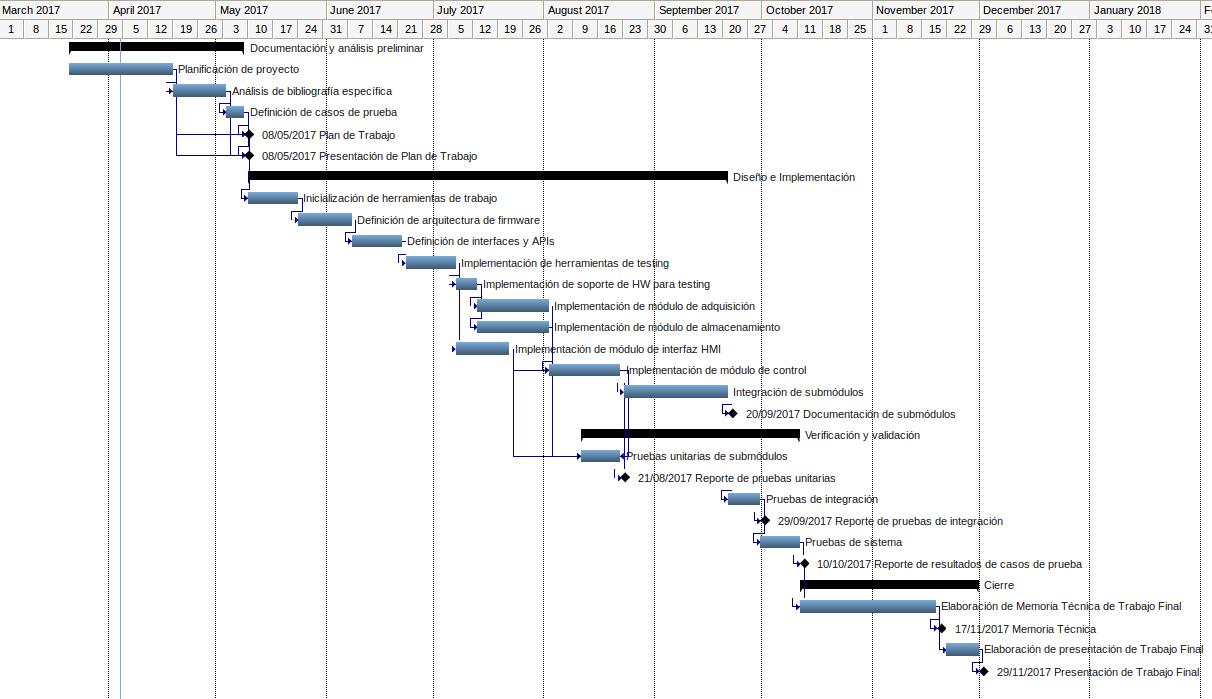
\includegraphics[height=.85\textheight]{./Figuras/Gantt-2.png}
%\caption{Ejemplo de diagrama de Gantt rotado}
%\label{fig:diagGantt}
%\end{figure}
%
%\end{landscape}
%
%\end{consigna}

%\begin{landscape}
\rotatebox{90}{%
\begin{ganttchart}[
	hgrid,
    vgrid={*4{dotted}, *3{red!50}}, %	vgrid,
	x unit=0.12cm,
	y unit chart=0.7cm,
	time slot format=isodate,
	time slot unit=day,
	bar/.append style={fill=blue!30},
	group/.append style={fill=blue!50},
	%link/.style={->, thick}
	]{2023-09-11}{2024-01-24}
	
	\gantttitlecalendar{year, month} \\
			\ganttmilestone{0. Acta de Constitución}{2023-09-11}\\
		\ganttgroup{1 Gestión del Proyecto}{2023-09-11}{2023-10-13} \\
		\ganttbar[name=11]{1.1 Generación de requerimientos}{2023-09-11}{2023-09-15} \\
		\ganttbar[name=12]{1.2 Planificación del proyecto}{2023-09-18}{2023-09-29} \\
		\ganttbar{1.3 Planificación de entregables}{2023-10-02}{2023-10-04} \\
		\ganttbar{1.4 Revisión y ajustes}{2023-10-04}{2023-10-13} \\
			\ganttmilestone{1.5 Proyecto de tesis}{2023-10-13} \\
	
	\ganttgroup{2 Diseño General}{2023-10-16}{2023-11-03} \\
		\ganttbar{2.1 Ajuste al diseño conceptual}{2023-10-16}{2023-10-18} \\
		\ganttbar{2.2 Diagramas de flujo}{2023-10-18}{2023-10-25} \\
		\ganttbar{2.3 Revisión y ajustes de diseño}{2023-10-25}{2023-11-03} \\
	
	\ganttgroup{3 Construcción del hardware}{2023-11-06}{2023-12-15} \\
		\ganttbar{3.1 Selección de componentes}{2023-11-06}{2023-11-10} \\
		\ganttbar{3.2 Diseño de circuitos}{2023-11-13}{2023-11-24} \\
		\ganttbar{3.3 Montaje y soldadura}{2023-11-27}{2023-12-06} \\
		\ganttbar{3.4 Pruebas iniciales}{2023-12-06}{2023-12-15} \\
	
	\ganttgroup{4 Diseño del firmware}{2023-12-18}{2024-01-24} \\
		\ganttbar{4.1 Diseño de arquitectura}{2023-12-18}{2023-12-22} \\
		\ganttbar{4.2 Implementación de MP2,5}{2023-12-25}{2024-01-03} \\
		\ganttbar{4.3 Almacenamiento y comunicación}{2024-01-03}{2024-01-12} \\
		\ganttbar{4.4 Funciones auxiliares}{2024-01-15}{2024-01-24} 
	
	\ganttlink[]{11}{12}
	
\end{ganttchart}
}
\newpage
\rotatebox{90}{%
\begin{ganttchart}[
	hgrid,
%vgrid,
 vgrid={*4{dotted}, *3{red!50}}, %	vgrid,
x unit=0.14cm,
y unit chart=0.7cm,
time slot format=isodate,
time slot unit=day,
bar/.append style={fill=blue!30},
group/.append style={fill=blue!50},
bar/.append style={fill=blue!30, bar label node/.append style={above=3pt}},
%include title in canvas=false,
%inline,
milestone inline label node/.append style={left=5mm}
%link/.style={->, thick}
%link label font=\small\bfseries\color{purple}
link/.style={|-to, line width=0.5pt, blue},
    bar inline label node/.style={
	anchor=east,
	xshift=+4.5cm,
	yshift=0.4cm,
}
]{2024-01-22}{2024-05-28}
	
	\gantttitlecalendar{year, month} \\
	
	\ganttgroup{5 Realización de pruebas}{2024-01-24}{2024-02-21} \\
		\ganttbar[name=51]{5.1 Diseño de casos de prueba}{2024-01-24}{2024-01-31} \\
		\ganttbar[name=52]{5.2 Ejecución de pruebas}{2024-01-31}{2024-02-14} \\
		\ganttbar[name=53]{5.3 Análisis de resultados}{2024-02-14}{2024-02-21} \\
		
	\ganttgroup{6 Ajustes finales}{2024-02-21}{2024-03-06} \\
		\ganttbar[name=61]{6.1 Depuración de errores}{2024-02-21}{2024-02-28} \\
		\ganttbar{6.2 Ajustes de performance}{2024-02-28}{2024-03-06} \\
			\ganttmilestone{6.3 Prototipo funcional}{2024-03-06} \\
		
	\ganttgroup{7 Generación escrito y manuales}{2024-03-06}{2024-05-08} \\
		\ganttbar{7.1 Marco teórico}{2024-03-06}{2024-03-20} \\
		\ganttbar{7.2 Metodología}{2024-03-20}{2024-03-27} \\
		\ganttbar{7.3 Implementación}{2024-03-27}{2024-04-03} \\
		\ganttbar{7.4 Resultados y conclusiones}{2024-04-03}{2024-04-10} \\
		\ganttbar{7.5 Introducción, resumen y otros}{2024-04-10}{2024-04-19} \\
		\ganttbar{7.6 Manual de usuario}{2024-04-22}{2024-04-26} \\
		\ganttbar{7.7 Manual técnico}{2024-04-29}{2024-05-08} \\
			\ganttmilestone{7.8 Manual técnico}{2024-05-08} \\
	
	\ganttgroup{8 Entregas del trabajo final}{2024-05-08}{2024-05-22} \\
		\ganttbar{8.1 Preparación de la presentación}{2024-05-08}{2024-05-22} \\
		\ganttbar{8.2 Presentación del trabajo final}{2024-05-22}{2024-05-22} \\
			\ganttmilestone{8.3 Informe final y presentación}{2024-05-22}
	
	\ganttlink[]{51}{52}
	\ganttlink[]{52}{53}
	\ganttlink[]{53}{61}

\end{ganttchart}
%\end{landscape}
}


% TODO: \usepackage{graphicx} required

%\includegraphics[width=0.9\textwidth, angle=270]{../planner/salida}





%\begin{consigna}{red}
%
%Existen muchos programas y recursos \textit{online} para hacer diagramas de Gantt, entre los cuales destacamos:
%
%\begin{itemize}
%\item Planner
%\item GanttProject
%\item Trello + \textit{plugins}. En el siguiente link hay un tutorial oficial: \\ \url{https://blog.trello.com/es/diagrama-de-gantt-de-un-proyecto}
%\item Creately, herramienta online colaborativa. \\\url{https://creately.com/diagram/example/ieb3p3ml/LaTeX}
%\item Se puede hacer en latex con el paquete \textit{pgfgantt}\\ \url{http://ctan.dcc.uchile.cl/graphics/pgf/contrib/pgfgantt/pgfgantt.pdf}
%\end{itemize}
%
%Pegar acá una captura de pantalla del diagrama de Gantt, cuidando que la letra sea suficientemente grande como para ser legible. 
%Si el diagrama queda demasiado ancho, se puede pegar primero la ``tabla'' del Gantt y luego pegar la parte del diagrama de barras del diagrama de Gantt.
%
%Configurar el software para que en la parte de la tabla muestre los códigos del EDT (WBS).\\
%Configurar el software para que al lado de cada barra muestre el nombre de cada tarea.\\
%Revisar que la fecha de finalización coincida con lo indicado en el Acta Constitutiva.
%
%En la figura \ref{fig:gantt}, se muestra un ejemplo de diagrama de Gantt realizado con el paquete de \textit{pgfgantt}. En la plantilla pueden ver el código que lo genera y usarlo de base para construir el propio.
%
%\begin{figure}[htbp]
%\begin{center}
%\begin{ganttchart}{1}{12}
%  \gantttitle{2020}{12} \\
%  \gantttitlelist{1,...,12}{1} \\
%  \ganttgroup{Group 1}{1}{7} \\
%  \ganttbar{Task 1}{1}{2} \\
%  \ganttlinkedbar{Task 2}{3}{7} \ganttnewline
%  \ganttmilestone{Milestone o hito}{7} \ganttnewline
%  \ganttbar{Final Task}{8}{12}
%  \ganttlink{elem2}{elem3}
%  \ganttlink{elem3}{elem4}
%\end{ganttchart}
%\end{center}
%\caption{Diagrama de Gantt de ejemplo}
%\label{fig:gantt}
%\end{figure}
%
%
%\begin{landscape}
%\begin{figure}[htpb]
%\centering 
%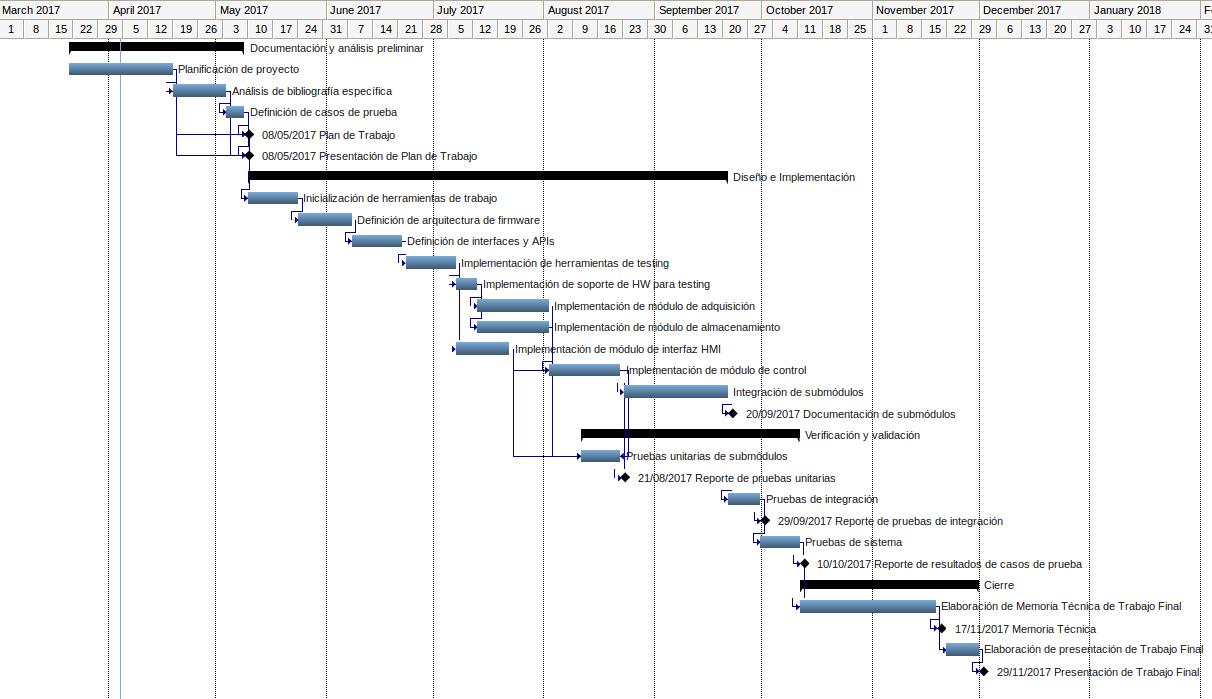
\includegraphics[height=.85\textheight]{./Figuras/Gantt-2.png}
%\caption{Ejemplo de diagrama de Gantt rotado}
%\label{fig:diagGantt}
%\end{figure}
%
%\end{landscape}
%
%\end{consigna}

%\begin{landscape}
\rotatebox{90}{%
\begin{ganttchart}[
	hgrid,
    vgrid={*4{dotted}, *3{red!50}}, %	vgrid,
	x unit=0.12cm,
	y unit chart=0.7cm,
	time slot format=isodate,
	time slot unit=day,
	bar/.append style={fill=blue!30},
	group/.append style={fill=blue!50},
	%link/.style={->, thick}
	]{2023-09-11}{2024-01-24}
	
	\gantttitlecalendar{year, month} \\
			\ganttmilestone{0. Acta de Constitución}{2023-09-11}\\
		\ganttgroup{1 Gestión del Proyecto}{2023-09-11}{2023-10-13} \\
		\ganttbar[name=11]{1.1 Generación de requerimientos}{2023-09-11}{2023-09-15} \\
		\ganttbar[name=12]{1.2 Planificación del proyecto}{2023-09-18}{2023-09-29} \\
		\ganttbar{1.3 Planificación de entregables}{2023-10-02}{2023-10-04} \\
		\ganttbar{1.4 Revisión y ajustes}{2023-10-04}{2023-10-13} \\
			\ganttmilestone{1.5 Proyecto de tesis}{2023-10-13} \\
	
	\ganttgroup{2 Diseño General}{2023-10-16}{2023-11-03} \\
		\ganttbar{2.1 Ajuste al diseño conceptual}{2023-10-16}{2023-10-18} \\
		\ganttbar{2.2 Diagramas de flujo}{2023-10-18}{2023-10-25} \\
		\ganttbar{2.3 Revisión y ajustes de diseño}{2023-10-25}{2023-11-03} \\
	
	\ganttgroup{3 Construcción del hardware}{2023-11-06}{2023-12-15} \\
		\ganttbar{3.1 Selección de componentes}{2023-11-06}{2023-11-10} \\
		\ganttbar{3.2 Diseño de circuitos}{2023-11-13}{2023-11-24} \\
		\ganttbar{3.3 Montaje y soldadura}{2023-11-27}{2023-12-06} \\
		\ganttbar{3.4 Pruebas iniciales}{2023-12-06}{2023-12-15} \\
	
	\ganttgroup{4 Diseño del firmware}{2023-12-18}{2024-01-24} \\
		\ganttbar{4.1 Diseño de arquitectura}{2023-12-18}{2023-12-22} \\
		\ganttbar{4.2 Implementación de MP2,5}{2023-12-25}{2024-01-03} \\
		\ganttbar{4.3 Almacenamiento y comunicación}{2024-01-03}{2024-01-12} \\
		\ganttbar{4.4 Funciones auxiliares}{2024-01-15}{2024-01-24} 
	
	\ganttlink[]{11}{12}
	
\end{ganttchart}
}
\newpage
\rotatebox{90}{%
\begin{ganttchart}[
	hgrid,
%vgrid,
 vgrid={*4{dotted}, *3{red!50}}, %	vgrid,
x unit=0.14cm,
y unit chart=0.7cm,
time slot format=isodate,
time slot unit=day,
bar/.append style={fill=blue!30},
group/.append style={fill=blue!50},
bar/.append style={fill=blue!30, bar label node/.append style={above=3pt}},
%include title in canvas=false,
%inline,
milestone inline label node/.append style={left=5mm}
%link/.style={->, thick}
%link label font=\small\bfseries\color{purple}
link/.style={|-to, line width=0.5pt, blue},
    bar inline label node/.style={
	anchor=east,
	xshift=+4.5cm,
	yshift=0.4cm,
}
]{2024-01-22}{2024-05-28}
	
	\gantttitlecalendar{year, month} \\
	
	\ganttgroup{5 Realización de pruebas}{2024-01-24}{2024-02-21} \\
		\ganttbar[name=51]{5.1 Diseño de casos de prueba}{2024-01-24}{2024-01-31} \\
		\ganttbar[name=52]{5.2 Ejecución de pruebas}{2024-01-31}{2024-02-14} \\
		\ganttbar[name=53]{5.3 Análisis de resultados}{2024-02-14}{2024-02-21} \\
		
	\ganttgroup{6 Ajustes finales}{2024-02-21}{2024-03-06} \\
		\ganttbar[name=61]{6.1 Depuración de errores}{2024-02-21}{2024-02-28} \\
		\ganttbar{6.2 Ajustes de performance}{2024-02-28}{2024-03-06} \\
			\ganttmilestone{6.3 Prototipo funcional}{2024-03-06} \\
		
	\ganttgroup{7 Generación escrito y manuales}{2024-03-06}{2024-05-08} \\
		\ganttbar{7.1 Marco teórico}{2024-03-06}{2024-03-20} \\
		\ganttbar{7.2 Metodología}{2024-03-20}{2024-03-27} \\
		\ganttbar{7.3 Implementación}{2024-03-27}{2024-04-03} \\
		\ganttbar{7.4 Resultados y conclusiones}{2024-04-03}{2024-04-10} \\
		\ganttbar{7.5 Introducción, resumen y otros}{2024-04-10}{2024-04-19} \\
		\ganttbar{7.6 Manual de usuario}{2024-04-22}{2024-04-26} \\
		\ganttbar{7.7 Manual técnico}{2024-04-29}{2024-05-08} \\
			\ganttmilestone{7.8 Manual técnico}{2024-05-08} \\
	
	\ganttgroup{8 Entregas del trabajo final}{2024-05-08}{2024-05-22} \\
		\ganttbar{8.1 Preparación de la presentación}{2024-05-08}{2024-05-22} \\
		\ganttbar{8.2 Presentación del trabajo final}{2024-05-22}{2024-05-22} \\
			\ganttmilestone{8.3 Informe final y presentación}{2024-05-22}
	
	\ganttlink[]{51}{52}
	\ganttlink[]{52}{53}
	\ganttlink[]{53}{61}

\end{ganttchart}
%\end{landscape}
}


% TODO: \usepackage{graphicx} required

%\includegraphics[width=0.9\textwidth, angle=270]{../planner/salida}





%\begin{consigna}{red}
%
%Existen muchos programas y recursos \textit{online} para hacer diagramas de Gantt, entre los cuales destacamos:
%
%\begin{itemize}
%\item Planner
%\item GanttProject
%\item Trello + \textit{plugins}. En el siguiente link hay un tutorial oficial: \\ \url{https://blog.trello.com/es/diagrama-de-gantt-de-un-proyecto}
%\item Creately, herramienta online colaborativa. \\\url{https://creately.com/diagram/example/ieb3p3ml/LaTeX}
%\item Se puede hacer en latex con el paquete \textit{pgfgantt}\\ \url{http://ctan.dcc.uchile.cl/graphics/pgf/contrib/pgfgantt/pgfgantt.pdf}
%\end{itemize}
%
%Pegar acá una captura de pantalla del diagrama de Gantt, cuidando que la letra sea suficientemente grande como para ser legible. 
%Si el diagrama queda demasiado ancho, se puede pegar primero la ``tabla'' del Gantt y luego pegar la parte del diagrama de barras del diagrama de Gantt.
%
%Configurar el software para que en la parte de la tabla muestre los códigos del EDT (WBS).\\
%Configurar el software para que al lado de cada barra muestre el nombre de cada tarea.\\
%Revisar que la fecha de finalización coincida con lo indicado en el Acta Constitutiva.
%
%En la figura \ref{fig:gantt}, se muestra un ejemplo de diagrama de Gantt realizado con el paquete de \textit{pgfgantt}. En la plantilla pueden ver el código que lo genera y usarlo de base para construir el propio.
%
%\begin{figure}[htbp]
%\begin{center}
%\begin{ganttchart}{1}{12}
%  \gantttitle{2020}{12} \\
%  \gantttitlelist{1,...,12}{1} \\
%  \ganttgroup{Group 1}{1}{7} \\
%  \ganttbar{Task 1}{1}{2} \\
%  \ganttlinkedbar{Task 2}{3}{7} \ganttnewline
%  \ganttmilestone{Milestone o hito}{7} \ganttnewline
%  \ganttbar{Final Task}{8}{12}
%  \ganttlink{elem2}{elem3}
%  \ganttlink{elem3}{elem4}
%\end{ganttchart}
%\end{center}
%\caption{Diagrama de Gantt de ejemplo}
%\label{fig:gantt}
%\end{figure}
%
%
%\begin{landscape}
%\begin{figure}[htpb]
%\centering 
%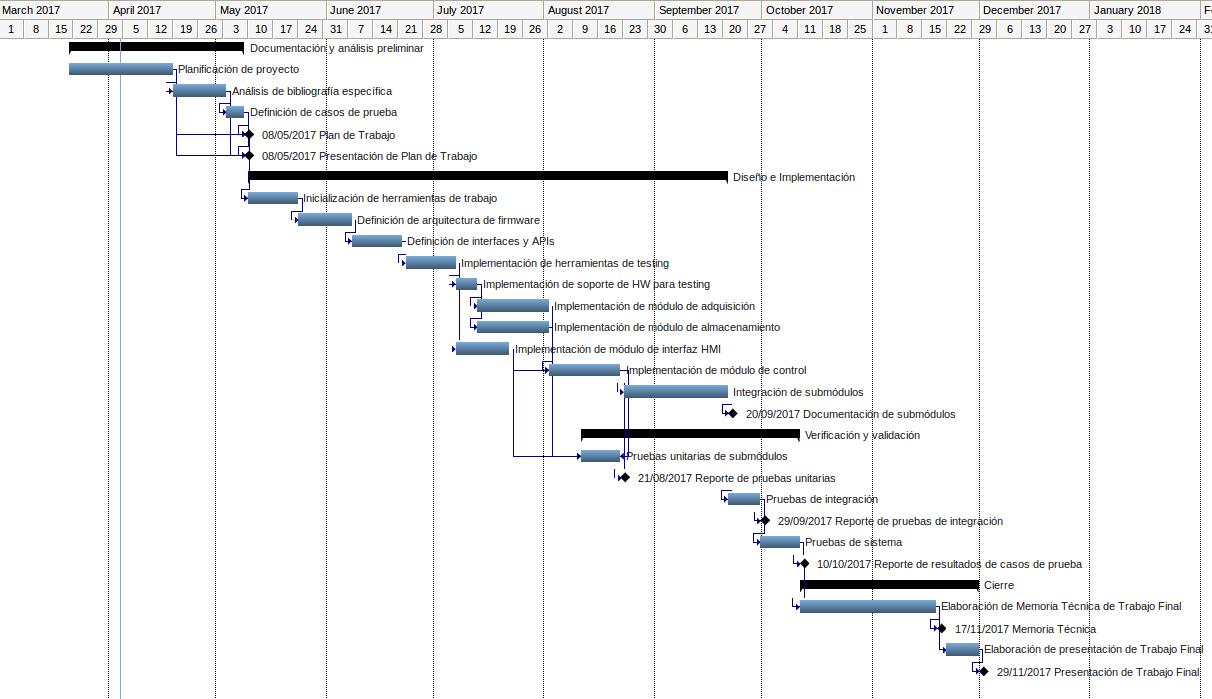
\includegraphics[height=.85\textheight]{./Figuras/Gantt-2.png}
%\caption{Ejemplo de diagrama de Gantt rotado}
%\label{fig:diagGantt}
%\end{figure}
%
%\end{landscape}
%
%\end{consigna}

%\begin{landscape}
\rotatebox{90}{%
\begin{ganttchart}[
	hgrid,
    vgrid={*4{dotted}, *3{red!50}}, %	vgrid,
	x unit=0.12cm,
	y unit chart=0.7cm,
	time slot format=isodate,
	time slot unit=day,
	bar/.append style={fill=blue!30},
	group/.append style={fill=blue!50},
	%link/.style={->, thick}
	]{2023-09-11}{2024-01-24}
	
	\gantttitlecalendar{year, month} \\
			\ganttmilestone{0. Acta de constitución}{2023-09-11}\\
		\ganttgroup{1 Gestión del proyecto}{2023-09-11}{2023-10-13} \\
		\ganttbar[name=11]{1.1 Generación de requerimientos}{2023-09-11}{2023-09-15} \\
		\ganttbar[name=12]{1.2 Planificación del proyecto}{2023-09-18}{2023-09-29} \\
		\ganttbar{1.3 Planificación de entregables}{2023-10-02}{2023-10-04} \\
		\ganttbar{1.4 Revisión y ajustes}{2023-10-04}{2023-10-13} \\
			\ganttmilestone{1.5 Proyecto de tesis}{2023-10-13} \\
	
	\ganttgroup{2 Diseño general}{2023-10-16}{2023-11-03} \\
		\ganttbar{2.1 Ajuste al diseño conceptual}{2023-10-16}{2023-10-18} \\
		\ganttbar{2.2 Diagramas de flujo}{2023-10-18}{2023-10-25} \\
		\ganttbar{2.3 Revisión y ajustes de diseño}{2023-10-25}{2023-11-03} \\
	
	\ganttgroup{3 Construcción del hardware}{2023-11-06}{2023-12-15} \\
		\ganttbar{3.1 Selección de componentes}{2023-11-06}{2023-11-10} \\
		\ganttbar{3.2 Diseño de circuitos}{2023-11-13}{2023-11-24} \\
		\ganttbar{3.3 Montaje y soldadura}{2023-11-27}{2023-12-06} \\
		\ganttbar{3.4 Pruebas iniciales}{2023-12-06}{2023-12-15} \\
	
	\ganttgroup{4 Diseño del firmware}{2023-12-18}{2024-01-24} \\
		\ganttbar{4.1 Diseño de arquitectura}{2023-12-18}{2023-12-22} \\
		\ganttbar{4.2 Implementación de MP2,5}{2023-12-25}{2024-01-03} \\
		\ganttbar{4.3 Almacenamiento y comunicación}{2024-01-03}{2024-01-12} \\
		\ganttbar{4.4 Funciones auxiliares}{2024-01-15}{2024-01-24} 
	
	\ganttlink[]{11}{12}
	
\end{ganttchart}
}
\newpage
\rotatebox{90}{%
\begin{ganttchart}[
	hgrid,
%vgrid,
 vgrid={*4{dotted}, *3{red!50}}, %	vgrid,
x unit=0.14cm,
y unit chart=0.7cm,
time slot format=isodate,
time slot unit=day,
bar/.append style={fill=blue!30},
group/.append style={fill=blue!50},
bar/.append style={fill=blue!30, bar label node/.append style={above=3pt}},
%include title in canvas=false,
%inline,
milestone inline label node/.append style={left=5mm}
%link/.style={->, thick}
%link label font=\small\bfseries\color{purple}
link/.style={|-to, line width=0.5pt, blue},
    bar inline label node/.style={
	anchor=east,
	xshift=+4.5cm,
	yshift=0.4cm,
}
]{2024-01-22}{2024-05-28}
	
	\gantttitlecalendar{year, month} \\
	
	\ganttgroup{5 Realización de pruebas}{2024-01-24}{2024-02-21} \\
		\ganttbar[name=51]{5.1 Diseño de casos de prueba}{2024-01-24}{2024-01-31} \\
		\ganttbar[name=52]{5.2 Ejecución de pruebas}{2024-01-31}{2024-02-14} \\
		\ganttbar[name=53]{5.3 Análisis de resultados}{2024-02-14}{2024-02-21} \\
		
	\ganttgroup{6 Ajustes finales}{2024-02-21}{2024-03-06} \\
		\ganttbar[name=61]{6.1 Depuración de errores}{2024-02-21}{2024-02-28} \\
		\ganttbar{6.2 Ajustes de performance}{2024-02-28}{2024-03-06} \\
			\ganttmilestone{6.3 Prototipo funcional}{2024-03-06} \\
		
	\ganttgroup{7 Generación escrito y manuales}{2024-03-06}{2024-05-08} \\
		\ganttbar{7.1 Marco teórico}{2024-03-06}{2024-03-20} \\
		\ganttbar{7.2 Metodología}{2024-03-20}{2024-03-27} \\
		\ganttbar{7.3 Implementación}{2024-03-27}{2024-04-03} \\
		\ganttbar{7.4 Resultados y conclusiones}{2024-04-03}{2024-04-10} \\
		\ganttbar{7.5 Introducción, resumen y otros}{2024-04-10}{2024-04-19} \\
		\ganttbar{7.6 Manual de usuario}{2024-04-22}{2024-04-26} \\
		\ganttbar{7.7 Manual técnico}{2024-04-29}{2024-05-08} \\
			\ganttmilestone{7.8 Manual técnico}{2024-05-08} \\
	
	\ganttgroup{8 Entregas del trabajo final}{2024-05-08}{2024-05-22} \\
		\ganttbar{8.1 Proceso de cierre}{2024-05-08}{2024-05-22} \\
		\ganttbar{8.2 Presentación del trabajo final}{2024-05-22}{2024-05-22} \\
			\ganttmilestone{8.3 Informe final y presentación}{2024-05-22}
	
	\ganttlink[]{51}{52}
	\ganttlink[]{52}{53}
	\ganttlink[]{53}{61}

\end{ganttchart}
%\end{landscape}
}


% TODO: \usepackage{graphicx} required

%\includegraphics[width=0.9\textwidth, angle=270]{../planner/salida}



